\documentclass{article}[18pt]
\ProvidesPackage{format}
%Page setup
\usepackage[utf8]{inputenc}
\usepackage[margin=0.7in]{geometry}
\usepackage{parselines} 
\usepackage[english]{babel}
\usepackage{fancyhdr}
\usepackage{titlesec}
\hyphenpenalty=10000

\pagestyle{fancy}
\fancyhf{}
\rhead{Sam Robbins}
\rfoot{Page \thepage}

%Characters
\usepackage{amsmath}
\usepackage{amssymb}
\usepackage{gensymb}
\newcommand{\R}{\mathbb{R}}

%Diagrams
\usepackage{pgfplots}
\usepackage{graphicx}
\usepackage{tabularx}
\usepackage{relsize}
\pgfplotsset{width=10cm,compat=1.9}
\usepackage{float}

%Length Setting
\titlespacing\section{0pt}{14pt plus 4pt minus 2pt}{0pt plus 2pt minus 2pt}
\newlength\tindent
\setlength{\tindent}{\parindent}
\setlength{\parindent}{0pt}
\renewcommand{\indent}{\hspace*{\tindent}}

%Programming Font
\usepackage{courier}
\usepackage{listings}
\usepackage{pxfonts}

%Lists
\usepackage{enumerate}
\usepackage{enumitem}

% Networks Macro
\usepackage{tikz}


% Commands for files converted using pandoc
\providecommand{\tightlist}{%
	\setlength{\itemsep}{0pt}\setlength{\parskip}{0pt}}
\usepackage{hyperref}

% Get nice commands for floor and ceil
\usepackage{mathtools}
\DeclarePairedDelimiter{\ceil}{\lceil}{\rceil}
\DeclarePairedDelimiter{\floor}{\lfloor}{\rfloor}

% Allow itemize to go up to 20 levels deep (just change the number if you need more you madman)
\usepackage{enumitem}
\setlistdepth{20}
\renewlist{itemize}{itemize}{20}

% initially, use dots for all levels
\setlist[itemize]{label=$\cdot$}

% customize the first 3 levels
\setlist[itemize,1]{label=\textbullet}
\setlist[itemize,2]{label=--}
\setlist[itemize,3]{label=*}

% Definition and Important Stuff
% Important stuff
\usepackage[framemethod=TikZ]{mdframed}

\newcounter{theo}[section]\setcounter{theo}{0}
\renewcommand{\thetheo}{\arabic{section}.\arabic{theo}}
\newenvironment{important}[1][]{%
	\refstepcounter{theo}%
	\ifstrempty{#1}%
	{\mdfsetup{%
			frametitle={%
				\tikz[baseline=(current bounding box.east),outer sep=0pt]
				\node[anchor=east,rectangle,fill=red!50]
				{\strut Important};}}
	}%
	{\mdfsetup{%
			frametitle={%
				\tikz[baseline=(current bounding box.east),outer sep=0pt]
				\node[anchor=east,rectangle,fill=red!50]
				{\strut Important:~#1};}}%
	}%
	\mdfsetup{innertopmargin=10pt,linecolor=red!50,%
		linewidth=2pt,topline=true,%
		frametitleaboveskip=\dimexpr-\ht\strutbox\relax
	}
	\begin{mdframed}[]\relax%
		\centering
		}{\end{mdframed}}



\newcounter{lem}[section]\setcounter{lem}{0}
\renewcommand{\thelem}{\arabic{section}.\arabic{lem}}
\newenvironment{defin}[1][]{%
	\refstepcounter{lem}%
	\ifstrempty{#1}%
	{\mdfsetup{%
			frametitle={%
				\tikz[baseline=(current bounding box.east),outer sep=0pt]
				\node[anchor=east,rectangle,fill=blue!20]
				{\strut Definition};}}
	}%
	{\mdfsetup{%
			frametitle={%
				\tikz[baseline=(current bounding box.east),outer sep=0pt]
				\node[anchor=east,rectangle,fill=blue!20]
				{\strut Definition:~#1};}}%
	}%
	\mdfsetup{innertopmargin=10pt,linecolor=blue!20,%
		linewidth=2pt,topline=true,%
		frametitleaboveskip=\dimexpr-\ht\strutbox\relax
	}
	\begin{mdframed}[]\relax%
		\centering
		}{\end{mdframed}}
\lhead{ADS - Rob Powell}
\usepackage{listings}
\usepackage{pxfonts}

\lstset{language=Python,
	basicstyle=\ttfamily,
	keywordstyle=\bfseries,
	showstringspaces=false,
	morekeywords={if, else, then, print, end, for, do, while},
	tabsize=4,
	mathescape=true
}

\begin{document}
\begin{center}
\underline{\huge Sorting}
\end{center}
\begin{center}
	{\large \textbf{Note that they're indexing from 1}}	
\end{center}
\section{Insertion Sort}

\begin{lstlisting}
InsertionSort $(a_1,...,a_n\in \mathbb{R}, n\geqslant 2)$
for j=2 to n do
	$x=a_j$
	i=j-1
	while i>0 and $a_i>x$ do
		$a_{i+1}=a_i$
		i=i-1
	end while
	$a_{i+1}=x$
end for
\end{lstlisting}
We know:
\begin{itemize}
	\item When j has a certain value, it insets the jth element into already sorted sequence $a_1,...,a_{j-1}$
	\item Can be proved correct by using invariant "after jth iteration first j+1 elements are in order" (not necessarily in the correct position for at the end of the sort)
	\item Running time between n-1 and $\dfrac{n(n-1)}{2}$  - worst case $\mathcal{O}(n^2)$
\end{itemize}
Method:
\begin{itemize}
	\item After the first n cycles, the first n+1 numbers are in order (not necessarily wrt the rest of the list)
	\item If there are repeats as the algorithm looks for strictly greater, suppose the list started with 2 twos, the algorithm would look at it as sorted. The order of repeated elements will not be changed. We call an algorithm that works like this \textbf{stable}
\end{itemize}
\section{Selection sort}
\begin{lstlisting}
SelectionSort $(a_1,...,a_n\in \mathbb{R}, n\geqslant 2)$
for i=1 to n-1 do
	elem = $a_i$
	pos = i
	for j=i+1 to n do
		if $a_j$<elem then
			elem=$a_j$
			pos=j
		end if
	end for
	swap $a_i$ and $a_{pos}$
end for			
\end{lstlisting}
How does it work?
\begin{itemize}
	\item Invariant: after ith iteration positions 1,...,i contain the overall i many smallest elements in order
	\item Not necessarily the first i elements
	\item In ith iteration of outer loop, we search the ith smallest element in remainder (positions $i+1,...,n$) of input and swap it into position i
	\begin{itemize}
		\item elem keeps track of the current idea of value ith smallest element
		\item pos keeps track of current idea of position of the ith smallest element
	\end{itemize}
\end{itemize}
Time Complexity:
$$\begin{aligned} \sum _ { i = 1 } ^ { n - 1 } \sum _ { j = i + 1 } ^ { n } 1 & = \sum _ { i = 1 } ^ { n - 1 } ( n - i ) \\ & = \left( \sum _ { i = 1 } ^ { n - 1 } n \right) - \left( \sum _ { i = 1 } ^ { n - 1 } i \right) \\ & = \frac { n ( n - 1 ) } { 2 } \\ & = O \left( n ^ { 2 } \right) \end{aligned}$$
Always do the same number of comparisons, no best or worst case, always takes the same number of comparisons for a list of any given length\\
\\
This algorithm is unstable, the order of repeated elements will not be preserved
\section{Bubble sort}
\begin{lstlisting}
BubbleSort-1 $(a_1,...,a_n\in \mathbb{R}, n\geqslant 2)$
for i=1 to n-2 do
	for j=1 to n-1 do
		if $a_j>a_{j+1}$ then
			swap $a_j$ and $a_{j+1}$
		end if
	end for
end for		
\end{lstlisting}
This can be improved by keeping track of whether or not an element was swapped
\begin{lstlisting}
BubbleSort-1 $(a_1,...,a_n\in \mathbb{R}, n\geqslant 2)$
for i=1 to n-1 do
	swaps=0
	for j=1 to n-1 do
		if $a_j>a_{j+1}$ then
			swap $a_j$ and $a_{j+1}$
			swaps=swaps+1
		end if
	end for
	if swaps ==0 then
		break
	end if
end for		
\end{lstlisting}
This algorithm is stable
\subsection{Correctness}
A sequence $a_1,...a_n$ is sorted if for every adjacent pair $a_i,a_{i+1}$ we have $a_i\leqslant a_{i+1}$\\
Bubble sort achieves just that\\
Good way to think about it: the ith iteration of the outer loop bubbles the ith largest element to where it belongs
\subsection{Time}
$$\begin{aligned}  { \sum _ { i = 1 } ^ { n - 1 } \sum _ { j = 1 } ^ { n - 1 } 1 } & { = \sum _ { i = 1 } ^ { n - 1 } ( n - 1 ) } \\ { } & { = ( n - 1 ) ^ { 2 } = \mathcal{O} \left( n ^ { 2 } \right) } \end{aligned}$$
\section{MergeSort}
The basic idea is simple
\begin{itemize}
	\item If given sequence of no more than one element then we're done
	\item Otherwise (Length$>1$) split sequence into two shorter sequences of equal lenth, sort them recursively and merge the two resulting sequences
\end{itemize}
Assumption:
\begin{itemize}
	\item Length of top level input sequence is a power of two
	\item This allows for nice splitting into equally sized sub problems as they can all reduce to $2\times 1$
\end{itemize}
\begin{lstlisting}
list MergeSort (list m)
if length(m) $\leqslant$ 1 then
	return m
end if
int middle = length(m) / 2
list left, right, leftsorted, rightsorted

left = m[1..middle]
right = m[middle+1..length(m)]

leftsorted = MergeSort(left)
rightsorted = MergeSort(right)

return Merge(leftsorted, rightsorted)


\end{lstlisting}
This depth first approach is the easiest way to program it

\begin{itemize}
	\item There can be issues here with recursion depth as all the data is stored in memory, so some computers/programming languages will be unable to do it
	\item Note that this keeps a copy of the original data
\end{itemize}




\subsection{How to merge two sorted sequences}
\begin{itemize}
	\item Also simple
	\item Suppose two sorted sequences given as arguments, say left and right
	\item Start with initially empty result sequence
	\item If both left and right aren't empty look at the leftmost element from each, say $l_1$ and $r_1$
	\item If $l_1<r_1$ then append $l_1$ to the result (and remove it from left) otherwise append $r_1$ to result (and remove it from right)
	\item If either left or right is empty, append the entire other one to the result
	\item Repeat until both empty
\end{itemize}
\newpage
\begin{lstlisting}
list MergeSort (list left, list right)

list result
while length(left)>0 or length(right)>0 do
	if length(left)>0 and length(right)>0 then
		if first(left) $\leqslant$ first(right) then
			append first(left) to result
			left = rest(left)
		else
		#Keeping extra copies of the data in the result array
			append first(right) to result
			right = rest(right)
		end if
	else if length(left)>0 then
		append left to result
		left = empty list
	else 	# Length(right) $>$ 0
		append right to result
		right = empty list
	end if
end while
return result
\end{lstlisting}
\begin{itemize}
	\item Best case is for merging two sublists length n is n, where the 1st list are all smaller than the 2nd list
	\item In worst case the lists will be empty upon reaching the last element of both
	\begin{itemize}
		\item Alternating inputs in sublists (1,3,5,7) and (2,4,6,8) for example
	\end{itemize}
\end{itemize}
Mergesort:
\begin{itemize}
	\item is probably the simplest recursive sorting algorithm
	\item It's bad cases are a lot less bad than those of some other sorting algorithms
	\item It's good cases, however may be worse than some algorithms
	\item More technically, MergeSort always requires $n\log (n)$ steps to sort any n numbers
	\item Some of the above can get away with $\approx n$ in particularly nice, but \textbf{will} require $\approx n^2$ for others
	\item $n^2$ is a lot worse than $n\log(n)$
\end{itemize}
\section{QuickSort}
Note that this algorithm is all in place\\
\\
This is an example of divide and conquer
\begin{itemize}
	\item Does the hard work at the start, unlike merge sort
	\item Split input into two parts
	\item Recursively sort then, one after the other
	\item Concatenate the resulting, sorted subsequences
\end{itemize}
Method:
\begin{itemize}
	\item At the beginning of each recursive call, QuickSort picks one element from the current sequence, the \textbf{pivot}
	\item The partitioning will be done wrt to the pivot
	\begin{itemize}
		\item Each element smaller than the pivot goes into the left part
		\item Each element bigger than the pivot goes into the right part
		\item parts may have very different sizes
	\end{itemize}
	\item In some sense,
	\begin{itemize}
		\item MergeSort does the complicated part after the sorted subsequences come back from recursive calls
		\item QuickSort does its difficult bit prior to recursing. This means that simple concatenation afterwards is OK
	\end{itemize}
\end{itemize}
The basic flow is as follows:\\
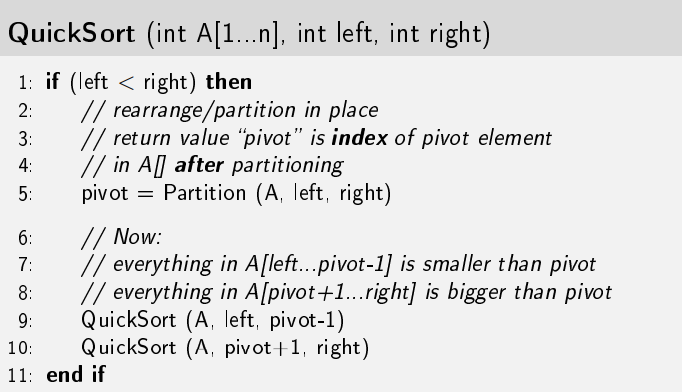
\includegraphics[scale=0.7]{QS}\\
This starts with left=1, right=n
\subsection{The partitioning function}
If the partition selected is the largest value, this is inefficient as one of the created sublists is empty\\
\\
The simplest method is to pick a fixed position in the current sequence, for example the right most, however this is not most efficient\\
\\
Partition moves everything smaller than the pivot, and everything bigger to the right. It does not sort\\
\\
This is how the partition procedure can be implemented\\
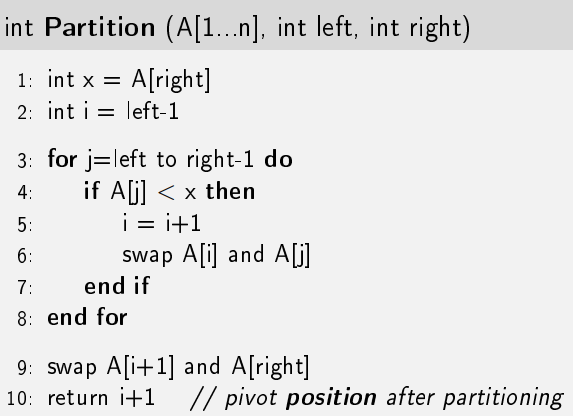
\includegraphics[scale=0.7]{partition}\\
This will swap values so that the values on the left are smaller than the pivot\\
It moves the pivot to just above the elements that have been swapped because they are less than 2
\subsection{Worst case}
Remember that if you are calling quicksort on two numbers, you will still have to make a quicksort on an empty space, due to the recursive nature of the algorithm. However, it will fail the if statement in the quick sort algorithm.\\
\\
The worst case will depend on how you choose your pivot.\\
\\
The worst case is where partition is called the maximum number of times. So the occasion where there are lists of length 0 and 1 should be delayed as much as possible.\\
\\
On choosing the right most element as the pivot, an already sorted list will be highly inefficient. This is because a right sublist would never be made\\
\\
The more evenly sized the sublists, the better the algorithm will perform\\
\\
This has a lower recursion depth than merge sort and does not keep copies of data. Slow memory fast CPU - quicksort. Fast memory slow CPU - mergesort
\subsection{Below length 4}
For example in quicksort, when the lengths of the sublists get less than 4, use a different algorithm.
\end{document}